\documentclass[11pt]{amsart}

\usepackage[T1]{fontenc}
\usepackage{lmodern}
\usepackage{amssymb,amsmath}
\usepackage{graphicx}
\usepackage{enumitem}
\usepackage[dvipsnames]{xcolor}
\usepackage[margin=1.15in]{geometry}
\usepackage[colorlinks=true,linkcolor=blue!50!black,citecolor=blue!50!black,urlcolor=blue!50!black]{hyperref}

\newtheorem{theorem}{Theorem}[section]
\newtheorem{proposition}[theorem]{Proposition}
\newtheorem{lemma}[theorem]{Lemma}
\newtheorem{corollary}[theorem]{Corollary}
\newtheorem{conjecture}[theorem]{Conjecture}
\theoremstyle{definition}
\newtheorem{definition}[theorem]{Definition}
\newtheorem{example}[theorem]{Example}
\theoremstyle{remark}
\newtheorem{remark}[theorem]{Remark}

\numberwithin{equation}{section}

\newcommand{\R}{\mathbb{R}}
\newcommand{\M}{\mathcal{M}}
\newcommand{\inter}{\operatorname{int}}
\hypersetup{pdftitle={Regular Morley tetrahedra from p-secting planes},pdfauthor={Deep Bhattacharjee}}
\providecommand{\doi}[1]{\url{https://doi.org/#1}}

\begin{document}

\title{Regular Morley tetrahedra from $p$-secting planes}

\author{Deep Bhattacharjee}
\address{Formerly, Electro-Gravitational Space Propulsion Laboratory (EGSPL),\newline Bhubaneswar, Odisha 751030, India}
\email{d.bhattacharjee@erl-forschung.de}
\email{itsdeep@live.com}
\urladdr{https://orcid.org/0000-0003-0466-750X}
\thanks{Corresponding author: \href{mailto:d.bhattacharjee@erl-forschung.de}{d.bhattacharjee@erl-forschung.de}; ORCID \href{https://orcid.org/0000-0003-0466-750X}{\mbox{0000-0003-0466-750X}}}

\subjclass[2020]{Primary 51M04; Secondary 51M20}
\keywords{Morley's theorem, Morley tetrahedron, $p$-secting plane, isosceles tetrahedron, disphenoid, dihedral angle}

\begin{abstract}
Tran replaced the trisecting planes of the Morley construction for a tetrahedron by $p$-secting planes, with one parameter for each pair of opposite edges, and conjectured that a regular Morley tetrahedron forces a pair of opposite edges whose four cross edges are equal. We show that every isosceles tetrahedron with three different edge lengths is a counterexample: its Morley tetrahedron is regular exactly when one vertex lies on one of four lines through the centre, and every such point occurs. When all three parameters equal $4$, only the regular tetrahedron remains.
\end{abstract}

\maketitle

\section{Introduction}

Morley's theorem says that the adjacent angle trisectors of a triangle meet in the vertices of an equilateral triangle~\cite{Mo,OB}. Tran~\cite{Tr21} carried the construction to a tetrahedron $ABCD$ by trisecting its six dihedral angles, and proved that the resulting Morley tetrahedron of an isosceles tetrahedron is again isosceles. In the same paper he replaced the trisecting planes by $p$-secting planes~\cite[Theorem~6]{Tr21}. We use the following form of the definition.

\begin{definition}\label{def:psect}
Let $XY$ be an edge of a tetrahedron, let $\theta_{XY}\in(0,\pi)$ be its interior dihedral angle, let $F$ be one of the two faces through $XY$, and let $p>1$. Let $F^+$ be the half-plane bounded by the line $XY$ that contains $F$, and let $H$ be the half-plane bounded by $XY$ that lies on the same side of the plane of $F$ as the tetrahedron and makes the angle $\theta_{XY}/p$ with $F^+$. The \emph{$p$-secting plane of $XY$ towards $F$} is the plane that contains $H$.
\end{definition}

Since $0<\theta_{XY}/p<\theta_{XY}$, the half-plane $H$ lies inside the dihedral angle at $XY$. For $p=3$ this is the trisecting plane of $XY$ that is closer to $F$. For numbers $e,f,g>1$ we attach the parameter $e$ to the edges $AB$ and $CD$, $f$ to $BC$ and $AD$, and $g$ to $AC$ and $BD$, as in~\cite[Theorem~6]{Tr21}. The tetrahedron
\[
\M_{e,f,g}(ABCD)=A'B'C'D'
\]
is defined as follows: $A'$ is the common point of the three planes that are $p$-secting towards the face $BCD$ through the edges $CD$, $BD$ and $BC$, with $p$ equal to the parameter of the edge, so $p=e$, $p=g$ and $p=f$ respectively; $B'$, $C'$ and $D'$ are obtained in the same way from the faces $ACD$, $ABD$ and $ABC$. Proposition~\ref{prop:param} below shows that the three planes always meet in exactly one point. For $e=f=g=3$ this is Tran's Morley tetrahedron.\footnote{Tran's paper~\cite{Tr26a} states the definition by saying that a $p$-secting plane makes the angle $\theta_{XY}/p$ with \emph{one} of the two faces through $XY$. Remark~\ref{rem:reading} explains why the results below do not depend on which face the angle is measured from.}

Tran~\cite{Tr26a} recently showed that both converse conjectures of~\cite{Tr21} are false: there are tetrahedra $T_1$ (not isosceles) and $T_2$ (isosceles but not regular) whose Morley tetrahedra are regular. In both, some pair of opposite edges $AB$, $CD$ has its four \emph{cross edges} $AC$, $AD$, $BC$, $BD$ of equal length. He conjectured that a regular Morley tetrahedron always forces this~\cite[Conjecture~8.1]{Tr26a}, proved it for every tetrahedron with a nontrivial symmetry~\cite[Corollary~11.6]{Tr26a}, and stated the analogue for $p$-secting planes.

\begin{conjecture}[Tran {\cite[Conjecture~8.6]{Tr26a}}]\label{conj:tran}
Let $e,f,g>1$. If $\M_{e,f,g}(ABCD)$ is regular, then, after relabeling the vertices, $AC=AD=BC=BD$.
\end{conjecture}

Tran notes that his methods do not apply to parameters other than $e=f=g=3$, and he lists the decision of Conjecture~\ref{conj:tran} among his open problems~\cite[Section~18.5 and Problem~8 of Section~19]{Tr26a}. We show that the conjecture is false, already for isosceles tetrahedra, where it holds for $e=f=g=3$~\cite[Theorems~10.1 and~10.3]{Tr26a}.

A tetrahedron is \emph{isosceles} if its opposite edges have equal lengths. Every isosceles tetrahedron is congruent to one with vertices
\begin{equation}\label{eq:box}
A=(a,b,c),\quad B=(a,-b,-c),\quad C=(-a,b,-c),\quad D=(-a,-b,c),\qquad a,b,c>0,
\end{equation}
that is, to a tetrahedron inscribed in the box $[-a,a]\times[-b,b]\times[-c,c]$~\cite{Le,BK}; Lemma~\ref{lem:box} below gives a short proof, with the labels of the vertices preserved. Its edge lengths are
\begin{equation}\label{eq:edges}
AB=CD=2\sqrt{b^2+c^2},\qquad AC=BD=2\sqrt{a^2+c^2},\qquad AD=BC=2\sqrt{a^2+b^2}.
\end{equation}
Let $O$ be the origin, the centre of the box, and let $\ell_1,\ell_2,\ell_3,\ell_4$ be the lines through $O$ in the directions $(1,1,1)$, $(1,-1,-1)$, $(-1,1,-1)$, $(-1,-1,1)$.

\begin{theorem}\label{thm:main}
Let $ABCD$ be the isosceles tetrahedron~\eqref{eq:box}.
\begin{enumerate}[label=\textup{(\alph*)}]
\item For all $e,f,g>1$, the tetrahedron $\M_{e,f,g}(ABCD)$ is regular if and only if $A'\neq O$ and $A'$ lies on $\ell_1\cup\ell_2\cup\ell_3\cup\ell_4$.
\item Every point $X\ne O$ of $\ell_1\cup\ell_2\cup\ell_3\cup\ell_4$ in the interior of $ABCD$ is the vertex $A'$ of $\M_{e,f,g}(ABCD)$ for exactly one triple $(e,f,g)$ with $e,f,g>1$.
\end{enumerate}
\end{theorem}

Distinct points $X$ in part~(b) give distinct triples, and the interior points of $\ell_1$ already form an open segment through $O$ (Section~\ref{sec:iso}), so there are infinitely many such triples. Figure~\ref{fig:box} shows one of the regular Morley tetrahedra.

\begin{corollary}\label{cor:false}
Conjecture~\ref{conj:tran} is false. If $a$, $b$, $c$ are pairwise different, the tetrahedron~\eqref{eq:box} has three different edge lengths, no pair of its opposite edges has four equal cross edges, and $\M_{e,f,g}(ABCD)$ is regular for infinitely many triples $(e,f,g)$.
\end{corollary}

\begin{figure}[ht]
\centering
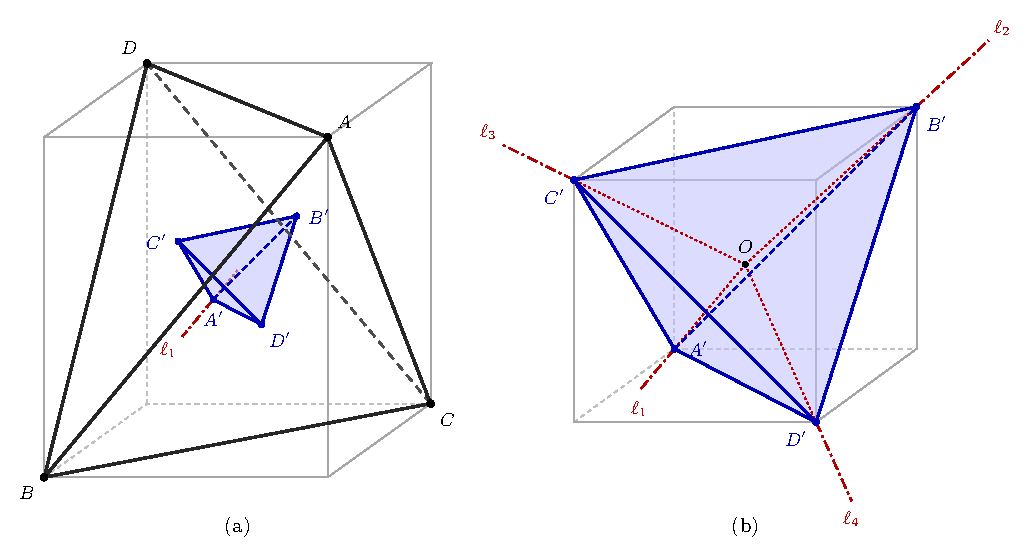
\includegraphics[width=\textwidth]{figures/box}
\caption{(a) An isosceles tetrahedron $ABCD$ in its box, and a regular tetrahedron $\M_{e,f,g}(ABCD)=A'B'C'D'$; its vertex $A'$ lies on the line $\ell_1$. (b) The same Morley tetrahedron, enlarged: its vertices are alternate vertices of a cube centred at $O$ with edges parallel to those of the box, and each of them lies on one of the lines $\ell_1,\dots,\ell_4$.}
\label{fig:box}
\end{figure}

The parameters can be written down in closed form. Here is an example in which all three parameters lie strictly between $2$ and $4$, and one in which two of them are equal to $4$.

\begin{example}\label{ex:123}
Take $(a,b,c)=(1,2,3)$, so that $AB=CD=2\sqrt{13}$, $AC=BD=2\sqrt{10}$ and $AD=BC=2\sqrt5$, and put
\[
e=\frac{\arccos(-23/49)}{\arctan\bigl(4\sqrt{13}/25\bigr)},\quad
f=\frac{\arccos(41/49)}{\arctan\bigl(20\sqrt5/297\bigr)},\quad
g=\frac{\arccos(31/49)}{\arctan\bigl(5\sqrt{10}/66\bigr)}.
\]
Then $2<e,f,g<4$, and $\M_{e,f,g}(ABCD)$ is the regular tetrahedron with vertices
\[
\tfrac27(-1,-1,-1),\quad \tfrac27(-1,1,1),\quad \tfrac27(1,-1,1),\quad \tfrac27(1,1,-1).
\]
\end{example}

\begin{example}\label{ex:44}
Take $(a,b,c)=(4,2,1)$, so that $AB=CD=2\sqrt5$, $AC=BD=2\sqrt{17}$ and $AD=BC=4\sqrt5$, and put $e=f=4$ and
\[
g=\frac{\arccos(13/21)}{\arctan\Bigl(2\sqrt{17}\big/\bigl(17+35\sqrt{5/21}\bigr)\Bigr)} .
\]
Then $2<g<4$, and $\M_{e,f,g}(ABCD)$ is the regular tetrahedron with vertices
\[
s(-1,-1,-1),\quad s(-1,1,1),\quad s(1,-1,1),\quad s(1,1,-1),\qquad\text{where } s=\tfrac52-\tfrac92\sqrt{5/21}>0.
\]
\end{example}

When the three parameters are equal, Theorem~\ref{thm:main} still applies, but the three conditions on $A'$ become harder to satisfy. For $e=f=g=3$, Tran showed that an isosceles tetrahedron with a regular Morley tetrahedron is regular or similar to $T_2$~\cite[Theorem~10.3]{Tr26a}. For quadrisecting planes the second possibility disappears.

\begin{theorem}\label{thm:four}
An isosceles tetrahedron $ABCD$ has a regular tetrahedron $\M_{4,4,4}(ABCD)$ if and only if $ABCD$ is regular.
\end{theorem}

Conjecture~\ref{conj:tran} for $e=f=g$ remains open; for $e=f=g=3$ it is Tran's Conjecture~8.1 in~\cite{Tr26a}.

Section~\ref{sec:construction} describes the construction through the distances to the faces; Proposition~\ref{prop:param} shows that $A'$ runs once through the interior of the tetrahedron as $(e,f,g)$ runs through $(1,\infty)^3$. Section~\ref{sec:iso} proves Theorem~\ref{thm:main}, Corollary~\ref{cor:false} and the two examples, and Section~\ref{sec:four} proves Theorem~\ref{thm:four}.

\section{The construction in terms of distances}\label{sec:construction}

Let $ABCD$ be a nondegenerate tetrahedron with volume $V$. For a vertex $X$ let $F_X$ be the opposite face, $S_X$ its area, $n_X$ its inward unit normal, and $d_X(P)$ the signed distance from a point $P$ to the plane of $F_X$, positive on the side of $X$. Each $d_X$ is an affine function. Splitting $ABCD$ into four tetrahedra with apex $P$ gives
\begin{equation}\label{eq:volume}
S_A\,d_A(P)+S_B\,d_B(P)+S_C\,d_C(P)+S_D\,d_D(P)=3V
\end{equation}
for $P$ in the tetrahedron, and hence for every $P\in\R^3$, since both sides are affine. The interior of $ABCD$ is the set where all four distances are positive. The interior dihedral angle between the faces $F_U$ and $F_W$, along the edge they share, satisfies $\cos\theta=-n_U\cdot n_W$.

For $\theta\in(0,\pi)$ and $p>1$ put
\[
R_p(\theta)=\frac{\sin\bigl((p-1)\theta/p\bigr)}{\sin(\theta/p)}.
\]

\begin{lemma}\label{lem:ratio}
Fix $\theta\in(0,\pi)$. Then $p\mapsto R_p(\theta)$ is a strictly increasing bijection from $(1,\infty)$ onto $(0,\infty)$, and $R_p(\theta)>1$ if and only if $p>2$. For $\rho>0$, the unique $p$ with $R_p(\theta)=\rho$ is $p=\theta/\varphi$, where $\varphi\in(0,\theta)$ is given by $\cot\varphi=(\rho+\cos\theta)/\sin\theta$.
\end{lemma}

\begin{proof}
Write $\varphi=\theta/p$, which decreases from $\theta$ to $0$ as $p$ increases from $1$ to $\infty$. Then
\[
R_p(\theta)=\frac{\sin(\theta-\varphi)}{\sin\varphi}=\sin\theta\cot\varphi-\cos\theta .
\]
Since $\sin\theta>0$ and $\cot$ decreases on $(0,\pi)$, this is a strictly decreasing function of $\varphi$; it tends to $0$ as $\varphi\to\theta$ and to $\infty$ as $\varphi\to0$. This gives the bijection and the formula for $p$. Finally $\sin(\theta-\varphi)-\sin\varphi=2\cos(\theta/2)\sin(\theta/2-\varphi)$, and $\cos(\theta/2)>0$, so $R_p(\theta)>1$ exactly when $\varphi<\theta/2$, that is, when $p>2$.
\end{proof}

\begin{figure}[ht]
\centering
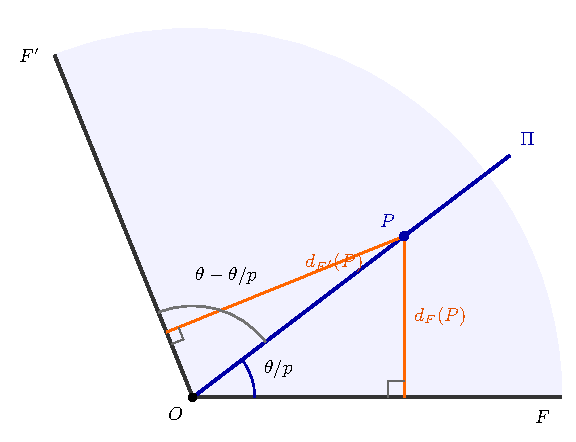
\includegraphics[width=0.56\textwidth]{figures/wedge}
\caption{A section perpendicular to an edge $XY$, which appears as the point $O$; the faces $F$ and $F'$ through $XY$ appear as two rays. The $p$-secting plane $\Pi$ of $XY$ towards $F$ makes the angle $\theta/p$ with $F$, and each of its points $P$ satisfies $d_{F'}(P)=R_p(\theta)\,d_F(P)$.}
\label{fig:wedge}
\end{figure}

\begin{lemma}\label{lem:plane}
Let $XY$ be an edge, and let $U$ and $W$ be the other two vertices, so that $XY=F_U\cap F_W$. For $p>1$, the $p$-secting plane of $XY$ towards $F_U$ is
\[
\{P\in\R^3:\ d_W(P)=R_p(\theta_{XY})\,d_U(P)\}.
\]
\end{lemma}

\begin{proof}
Let $\Pi$ be the $p$-secting plane and $\theta=\theta_{XY}$. The line $XY$ cuts $\Pi$ into two half-planes, and one of them lies inside the dihedral angle at $XY$. A point $P$ of that half-plane at distance $r$ from the line $XY$ has $d_U(P)=r\sin(\theta/p)$ and $d_W(P)=r\sin(\theta-\theta/p)$, because the half-plane makes the angles $\theta/p$ and $\theta-\theta/p$ with $F_U$ and $F_W$ (Figure~\ref{fig:wedge}). So the affine function $d_W-R_p(\theta)\,d_U$ vanishes on this half-plane and on the line $XY$. It is not constant, because $n_U$ and $n_W$ are linearly independent, so its zero set is a plane, and this plane is $\Pi$.
\end{proof}

For the vertex $A'$ the three edges are $CD=F_A\cap F_B$, $BD=F_A\cap F_C$ and $BC=F_A\cap F_D$, with parameters $e$, $g$ and $f$. By Lemma~\ref{lem:plane}, $A'$ is the common point of the three planes
\begin{equation}\label{eq:Aprime}
d_B=R_e(\theta_{CD})\,d_A,\qquad d_C=R_g(\theta_{BD})\,d_A,\qquad d_D=R_f(\theta_{BC})\,d_A ,
\end{equation}
and $B'$, $C'$, $D'$ are described in the same way.

\begin{proposition}\label{prop:param}
For all $e,f,g>1$ the three planes~\eqref{eq:Aprime} meet in exactly one point $A'$, and $A'$ lies in the interior of $ABCD$. The map $(e,f,g)\mapsto A'$ is a bijection from $(1,\infty)^3$ onto the interior of $ABCD$. Its inverse sends an interior point $P$ to the triple determined by
\begin{equation}\label{eq:inverse}
R_e(\theta_{CD})=\frac{d_B(P)}{d_A(P)},\qquad R_g(\theta_{BD})=\frac{d_C(P)}{d_A(P)},\qquad R_f(\theta_{BC})=\frac{d_D(P)}{d_A(P)} .
\end{equation}
The same holds for $B'$, $C'$ and $D'$.
\end{proposition}

\begin{proof}
The four normals $n_A,\dots,n_D$ span $\R^3$, so $P\mapsto(d_A(P),d_B(P),d_C(P),d_D(P))$ is an injective affine map from $\R^3$ to $\R^4$. By~\eqref{eq:volume} its image lies in the hyperplane $H=\{t\in\R^4: S_At_A+S_Bt_B+S_Ct_C+S_Dt_D=3V\}$, and since both are three-dimensional, the image is all of $H$. Write $\rho_e=R_e(\theta_{CD})$, $\rho_g=R_g(\theta_{BD})$ and $\rho_f=R_f(\theta_{BC})$; these are positive by Lemma~\ref{lem:ratio}. A point lies on the three planes~\eqref{eq:Aprime} exactly when its distance vector has the form $(\tau,\rho_e\tau,\rho_g\tau,\rho_f\tau)$, and such a vector lies in $H$ for exactly one $\tau$, namely
\[
\tau=\frac{3V}{S_A+\rho_eS_B+\rho_gS_C+\rho_fS_D}>0 .
\]
So the planes meet in exactly one point, and all its distances to the faces are positive. Conversely, for an interior point $P$ the three ratios in~\eqref{eq:inverse} are positive, and by Lemma~\ref{lem:ratio} each of them equals $R_p$ of the corresponding dihedral angle for exactly one $p>1$. With these parameters $P$ lies on the three planes~\eqref{eq:Aprime}, so $P=A'$; and no other triple gives $P$, again by Lemma~\ref{lem:ratio}.
\end{proof}

Two vertices of $\M_{e,f,g}(ABCD)$ can coincide only if a parameter equals $2$. For instance, a point $P=A'=B'$ satisfies $d_B(P)=R_e(\theta_{CD})\,d_A(P)$ and, since $B'$ lies on the $e$-secting plane of $CD$ towards $F_B$, also $d_A(P)=R_e(\theta_{CD})\,d_B(P)$; so $R_e(\theta_{CD})=1$ and $e=2$ by Lemma~\ref{lem:ratio}.

The symmetries we need permute the vertices by elements of the Klein group
\[
K=\{\mathrm{id},\ (A\,B)(C\,D),\ (A\,C)(B\,D),\ (A\,D)(B\,C)\}.
\]
Every element of $K$ maps each of the three pairs of opposite edges to itself; for instance $(A\,B)(C\,D)$ maps $AB$ and $CD$ to themselves, interchanges $AC$ and $BD$, and interchanges $AD$ and $BC$. So it preserves the parameter attached to every edge.

\begin{lemma}\label{lem:equiv}
Let $T_1$ be a second tetrahedron, let $\pi$ be a permutation of the labels $A,B,C,D$, and let $h$ be an isometry of $\R^3$ that maps each vertex $X$ of $ABCD$ to the vertex of $T_1$ with label $\pi(X)$. Let $e_1,f_1,g_1>1$ be parameters for $T_1$ such that, for all vertices $Y\ne Z$, the edge of $T_1$ with labels $\pi(Y)\pi(Z)$ carries the same parameter as $YZ$. Then $h$ maps the vertex $X'$ of $\M_{e,f,g}(ABCD)$ to the vertex of $\M_{e_1,f_1,g_1}(T_1)$ with label $\pi(X)$.
\end{lemma}

\begin{proof}
Write $d^1_X$ for the signed distances of $T_1$. The isometry $h$ maps the plane of $F_X$ to the plane of the face of $T_1$ opposite $\pi(X)$, and the side of $X$ to the side of $\pi(X)$, so $d^1_{\pi(X)}(h(P))=d_X(P)$ for every point $P$. It maps the inward normals of $ABCD$ to those of $T_1$, so it also preserves the dihedral angles: the angle of $T_1$ between the faces opposite $\pi(U)$ and $\pi(W)$ equals $\theta$ at $F_U\cap F_W$. By Lemma~\ref{lem:plane}, $X'$ satisfies $d_Y(X')=R_p(\theta)\,d_X(X')$ for the three vertices $Y\ne X$, where $\theta$ is the angle at $F_X\cap F_Y$ and $p$ is the parameter of that edge. Hence $h(X')$ satisfies $d^1_{\pi(Y)}(h(X'))=R_p(\theta)\,d^1_{\pi(X)}(h(X'))$, with the same $p$ and the same angle. By Lemma~\ref{lem:plane} and Proposition~\ref{prop:param} for $T_1$, $h(X')$ is the vertex of $\M_{e_1,f_1,g_1}(T_1)$ with label $\pi(X)$.
\end{proof}

We use Lemma~\ref{lem:equiv} in two ways: with $T_1=ABCD$, the same parameters and $\pi\in K$; and with $\pi$ the identity, when $h$ moves a tetrahedron into a standard position.

\begin{remark}\label{rem:reading}
If the angle $\theta_{XY}/p$ in Definition~\ref{def:psect} is measured from the other face through $XY$, the plane used for a given parameter $p$ is the one we use for $p/(p-1)$. The map $p\mapsto p/(p-1)$ is an involution of $(1,\infty)$, so the family of tetrahedra $\M_{e,f,g}(ABCD)$ is the same, with the parameters renamed. If instead one always takes the $p$-secting plane closer to the face, only parameters $p\ge2$ occur. In Examples~\ref{ex:123} and~\ref{ex:44} all parameters exceed $2$, so these examples disprove Conjecture~\ref{conj:tran} under each of these readings.
\end{remark}

\section{Isosceles tetrahedra}\label{sec:iso}

\begin{lemma}\label{lem:box}
Let $ABCD$ be an isosceles tetrahedron. There are $a,b,c>0$ and an isometry $h$ of $\R^3$ such that $h(A)$, $h(B)$, $h(C)$, $h(D)$ are the points~\eqref{eq:box}, in this order.
\end{lemma}

\begin{proof}
Put $O=\tfrac14(A+B+C+D)$ and
\[
u_1=\tfrac14(A+B-C-D),\qquad u_2=\tfrac14(A-B+C-D),\qquad u_3=\tfrac14(A-B-C+D).
\]
Then $A=O+u_1+u_2+u_3$, $B=O+u_1-u_2-u_3$, $C=O-u_1+u_2-u_3$ and $D=O-u_1-u_2+u_3$. Since $A-B=2(u_2+u_3)$ and $C-D=2(u_2-u_3)$, we get $|AB|^2-|CD|^2=16\,u_2\cdot u_3$; in the same way $|AC|^2-|BD|^2=16\,u_1\cdot u_3$ and $|AD|^2-|BC|^2=16\,u_1\cdot u_2$. So $u_1$, $u_2$, $u_3$ are pairwise orthogonal. A direct expansion gives $(B-A)\cdot\bigl((C-A)\times(D-A)\bigr)=-16\,u_1\cdot(u_2\times u_3)$, which is not zero, so none of the $u_i$ vanishes. With $a=|u_1|$, $b=|u_2|$, $c=|u_3|$, the vectors $u_1/a$, $u_2/b$, $u_3/c$ form an orthonormal basis, and the isometry $h(P)=\bigl((P-O)\cdot u_1/a,\ (P-O)\cdot u_2/b,\ (P-O)\cdot u_3/c\bigr)$ sends $A$ to $(a,b,c)$, $B$ to $(a,-b,-c)$, $C$ to $(-a,b,-c)$ and $D$ to $(-a,-b,c)$.
\end{proof}

From now on let $ABCD$ be the tetrahedron~\eqref{eq:box}, and write $\alpha=1/a$, $\beta=1/b$, $\gamma=1/c$ and $N=(\alpha^2+\beta^2+\gamma^2)^{1/2}$. For a point $P=(x,y,z)$ put
\begin{align*}
L_A(P)&=1+\alpha x+\beta y+\gamma z, & L_B(P)&=1+\alpha x-\beta y-\gamma z,\\
L_C(P)&=1-\alpha x+\beta y-\gamma z, & L_D(P)&=1-\alpha x-\beta y+\gamma z.
\end{align*}
Each $L_X$ vanishes at the three vertices other than $X$ and equals $4$ at $X$; hence $d_X=L_X/N$, and the inward normals are $n_A=(\alpha,\beta,\gamma)/N$, $n_B=(\alpha,-\beta,-\gamma)/N$, $n_C=(-\alpha,\beta,-\gamma)/N$, $n_D=(-\alpha,-\beta,\gamma)/N$. The dihedral angles at the edges of the face $F_A$ are therefore given by
\begin{equation}\label{eq:cos}
\cos\theta_{CD}=\frac{-\alpha^2+\beta^2+\gamma^2}{N^2},\qquad
\cos\theta_{BD}=\frac{\alpha^2-\beta^2+\gamma^2}{N^2},\qquad
\cos\theta_{BC}=\frac{\alpha^2+\beta^2-\gamma^2}{N^2}.
\end{equation}
The three half-turns about the coordinate axes,
\[
h_1(x,y,z)=(x,-y,-z),\qquad h_2(x,y,z)=(-x,y,-z),\qquad h_3(x,y,z)=(-x,-y,z),
\]
map the tetrahedron to itself and induce the permutations $(A\,B)(C\,D)$, $(A\,C)(B\,D)$ and $(A\,D)(B\,C)$.

\begin{proof}[Proof of Theorem~\ref{thm:main}]
(a) Let $A'=(x,y,z)$. Lemma~\ref{lem:equiv}, applied to $h_1$, $h_2$ and $h_3$, gives
\[
B'=(x,-y,-z),\qquad C'=(-x,y,-z),\qquad D'=(-x,-y,z).
\]
Hence
\[
|A'B'|=|C'D'|=2\sqrt{y^2+z^2},\quad |A'C'|=|B'D'|=2\sqrt{x^2+z^2},\quad |A'D'|=|B'C'|=2\sqrt{x^2+y^2}.
\]
If $A'=O$, the four points coincide. Otherwise the six distances are equal if and only if $x^2=y^2=z^2$, that is, if and only if $A'$ lies on one of the lines $\ell_i$; and then $A'$, $B'$, $C'$, $D'$ are alternate vertices of the cube $[-|x|,|x|]^3$, which form a regular tetrahedron.

(b) This is Proposition~\ref{prop:param} applied to the interior point $X$.
\end{proof}

For $0<t<1/(\alpha+\beta+\gamma)$ the point $-t(1,1,1)$ of $\ell_1$ is interior: $L_A(-t,-t,-t)=1-t(\alpha+\beta+\gamma)>0$, and $L_B$, $L_C$, $L_D$ exceed $L_A$ there by $2t(\beta+\gamma)$, $2t(\alpha+\gamma)$ and $2t(\alpha+\beta)$. By part~(b) each of these points is the vertex $A'$ of a regular Morley tetrahedron, and distinct points give distinct triples because the map of Proposition~\ref{prop:param} is injective.

\begin{proof}[Proof of Corollary~\ref{cor:false}]
If $a,b,c$ are pairwise different, so are $b^2+c^2$, $a^2+c^2$ and $a^2+b^2$, and by~\eqref{eq:edges} the tetrahedron has three different edge lengths, each shared by a pair of opposite edges. Under any labeling, the four cross edges of a pair of opposite edges are the two other pairs, so they have two different lengths. On the other hand, by Theorem~\ref{thm:main} and the paragraph above, $\M_{e,f,g}(ABCD)$ is regular for the infinitely many triples obtained from the points $-t(1,1,1)$ with $0<t<1/(\alpha+\beta+\gamma)$.
\end{proof}

For a point $X$ on $\ell_1$ the ratios in~\eqref{eq:inverse} take a simple form. If $X=-t(1,1,1)$ with $t>0$, then
\begin{gather*}
L_A(X)=1-t(\alpha+\beta+\gamma),\qquad L_B(X)-L_A(X)=2t(\beta+\gamma),\\
L_C(X)-L_A(X)=2t(\alpha+\gamma),\qquad L_D(X)-L_A(X)=2t(\alpha+\beta),
\end{gather*}
so that, for $0<t<1/(\alpha+\beta+\gamma)$ and with $\lambda=t/L_A(X)>0$,
\begin{equation}\label{eq:l1ratios}
\frac{d_B(X)}{d_A(X)}=1+2(\beta+\gamma)\lambda,\qquad
\frac{d_C(X)}{d_A(X)}=1+2(\alpha+\gamma)\lambda,\qquad
\frac{d_D(X)}{d_A(X)}=1+2(\alpha+\beta)\lambda .
\end{equation}
For $p=4$ the identity $\sin3u=\sin u\,(1+2\cos 2u)$ gives
\begin{equation}\label{eq:R4}
R_4(\theta)=1+2\cos(\theta/2),\qquad\text{so}\qquad R_4(\theta)-1=\sqrt{2(1+\cos\theta)} .
\end{equation}
Since $p\mapsto R_p(\theta)$ is increasing (Lemma~\ref{lem:ratio}), a parameter $p$ with $R_p(\theta)=\rho$ satisfies $p<4$ as soon as $(\rho-1)^2<2(1+\cos\theta)$, and $p>2$ as soon as $\rho>1$.

\begin{proof}[Proof of Example~\ref{ex:123}]
Here $(\alpha,\beta,\gamma)=(1,\tfrac12,\tfrac13)$ and $N^2=\tfrac{49}{36}$, so~\eqref{eq:cos} gives $\cos\theta_{CD}=-\tfrac{23}{49}$, $\cos\theta_{BD}=\tfrac{31}{49}$ and $\cos\theta_{BC}=\tfrac{41}{49}$, with sines $\tfrac{12\sqrt{13}}{49}$, $\tfrac{12\sqrt{10}}{49}$ and $\tfrac{12\sqrt5}{49}$. Take $X=-\tfrac27(1,1,1)$. Then $L_A(X)=\tfrac{10}{21}>0$, so $X$ is interior, $\lambda=\tfrac35$, and~\eqref{eq:l1ratios} gives the ratios $2$, $\tfrac{13}{5}$ and $\tfrac{14}{5}$. By Lemma~\ref{lem:ratio} the parameters are $\theta/\varphi$ with $\tan\varphi=\sin\theta/(\rho+\cos\theta)$:
\begin{gather*}
\tan\varphi_{CD}=\frac{12\sqrt{13}/49}{2-\frac{23}{49}}=\frac{4\sqrt{13}}{25},\qquad
\tan\varphi_{BD}=\frac{12\sqrt{10}/49}{\frac{13}{5}+\frac{31}{49}}=\frac{5\sqrt{10}}{66},\\
\tan\varphi_{BC}=\frac{12\sqrt5/49}{\frac{14}{5}+\frac{41}{49}}=\frac{20\sqrt5}{297}.
\end{gather*}
These are the stated values of $e$, $g$ and $f$; the three angles $\varphi$ lie in $(0,\pi/2)$, so the arctangents are the right branches. The three ratios exceed $1$, and $2(1+\cos\theta)$ equals $\tfrac{52}{49}$, $\tfrac{160}{49}$ and $\tfrac{180}{49}$ for the edges $CD$, $BD$ and $BC$, which exceed $1^2$, $(\tfrac85)^2$ and $(\tfrac95)^2$; so $2<e,f,g<4$. By Proposition~\ref{prop:param}, $A'=X$, and by Theorem~\ref{thm:main} and its proof the other vertices are $h_1(X)$, $h_2(X)$ and $h_3(X)$.
\end{proof}

\begin{proof}[Proof of Example~\ref{ex:44}]
Here $(\alpha,\beta,\gamma)=(\tfrac14,\tfrac12,1)$ and $N^2=\tfrac{21}{16}$, so $\cos\theta_{CD}=\tfrac{19}{21}$, $\cos\theta_{BD}=\tfrac{13}{21}$ and $\cos\theta_{BC}=-\tfrac{11}{21}$. By~\eqref{eq:R4}, $R_4(\theta_{CD})=1+4\sqrt{5/21}$ and $R_4(\theta_{BC})=1+2\sqrt{5/21}$. By~\eqref{eq:l1ratios}, with $\beta+\gamma=\tfrac32$ and $\alpha+\beta=\tfrac34$, both equations $e=4$ and $f=4$ say $\lambda=\tfrac43\sqrt{5/21}$. For this $\lambda$ the point $X=-t(1,1,1)$ with $t=\lambda/\bigl(1+\tfrac74\lambda\bigr)=\tfrac52-\tfrac92\sqrt{5/21}$ is interior, and the third ratio is $1+\tfrac52\lambda=1+\tfrac{10}{3}\sqrt{5/21}$. With $\sin\theta_{BD}=\tfrac{4\sqrt{17}}{21}$, Lemma~\ref{lem:ratio} gives
\[
\tan\varphi_{BD}=\frac{4\sqrt{17}/21}{1+\frac{10}{3}\sqrt{5/21}+\frac{13}{21}}=\frac{2\sqrt{17}}{17+35\sqrt{5/21}},
\]
which is the stated value of $g$. The third ratio exceeds $1$, and $(\tfrac{10}{3})^2\cdot\tfrac{5}{21}=\tfrac{500}{189}<\tfrac{612}{189}=2(1+\cos\theta_{BD})$, so $2<g<4$. Finally $s>0$ because $\tfrac{5}{21}<\tfrac{25}{81}$. As before, $A'=X$ and the Morley tetrahedron is regular.
\end{proof}

\section{Quadrisecting planes}\label{sec:four}

\begin{proof}[Proof of Theorem~\ref{thm:four}]
By Lemma~\ref{lem:box} there is an isometry $h$ that maps $A$, $B$, $C$, $D$ to the points~\eqref{eq:box}, in this order. By Lemma~\ref{lem:equiv}, with $\pi$ the identity and all parameters equal to $4$, $h$ maps $\M_{4,4,4}(ABCD)$ onto $\M_{4,4,4}$ of the image, and an isometry preserves regularity. So we may assume that $ABCD$ is the tetrahedron~\eqref{eq:box}. By~\eqref{eq:edges} it is regular if and only if $a=b=c$, that is, $\alpha=\beta=\gamma$.

Suppose first that $\alpha=\beta=\gamma$. By~\eqref{eq:cos} the edges $CD$, $BD$ and $BC$ have the same dihedral angle $\theta$, and since $d_X=L_X/N$, \eqref{eq:Aprime} says that $L_B=L_C=L_D=R_4(\theta)\,L_A$ at $A'=(x,y,z)$. Now $L_B-L_C=2\alpha(x-y)$ and $L_C-L_D=2\alpha(y-z)$, so $x=y=z$ and $A'$ lies on $\ell_1$. If $A'$ were $O$, then $L_A(A')=L_B(A')=1$ would give $R_4(\theta)=1$, while $R_4(\theta)>1$ by Lemma~\ref{lem:ratio}. So $A'\ne O$, and $\M_{4,4,4}(ABCD)$ is regular by Theorem~\ref{thm:main}.

Conversely, suppose that $\M_{4,4,4}(ABCD)$ is regular. By Theorem~\ref{thm:main}, $A'=X$ is a point $t\delta\neq O$, where $\delta$ is one of $\delta_1=(1,1,1)$, $\delta_2=(1,-1,-1)$, $\delta_3=(-1,1,-1)$, $\delta_4=(-1,-1,1)$. Put $\mu=t/L_A(X)\ne0$ and
\[
q_{CD}=\beta^2+\gamma^2,\qquad q_{BD}=\alpha^2+\gamma^2,\qquad q_{BC}=\alpha^2+\beta^2 .
\]
By~\eqref{eq:cos}, $1+\cos\theta_{CD}=2q_{CD}/N^2$, and similarly for the other two edges. A direct computation from the formulas for $L_X$ gives
\[
\frac{d_B(X)}{d_A(X)}-1=-2\mu\,w_{CD},\qquad \frac{d_C(X)}{d_A(X)}-1=-2\mu\,w_{BD},\qquad \frac{d_D(X)}{d_A(X)}-1=-2\mu\,w_{BC},
\]
where $(w_{CD},w_{BD},w_{BC})$ equals
\[
(\beta+\gamma,\ \alpha+\gamma,\ \alpha+\beta),\quad
(-\beta-\gamma,\ \alpha-\gamma,\ \alpha-\beta),\quad
(\beta-\gamma,\ -\alpha-\gamma,\ \beta-\alpha),\quad
(\gamma-\beta,\ \gamma-\alpha,\ -\alpha-\beta)
\]
for $\delta=\delta_1,\delta_2,\delta_3,\delta_4$ respectively. Since all parameters equal $4$, \eqref{eq:inverse} and~\eqref{eq:R4} give, for each of the three edges $E$ of $F_A$,
\[
4\mu^2w_E^2=2(1+\cos\theta_E)=\frac{4q_E}{N^2},\qquad\text{so}\qquad \frac{q_E}{w_E^2}=\mu^2N^2.
\]
In particular $w_E\ne0$, since $q_E>0$, and the three quotients $q_E/w_E^2$ are equal.

For $\delta=\delta_2$ this is impossible: $q_{CD}/w_{CD}^2=(\beta^2+\gamma^2)/(\beta+\gamma)^2<1$, while $q_{BD}/w_{BD}^2=(\alpha^2+\gamma^2)/(\alpha-\gamma)^2>1$. In the same way the edges $BD$ and $CD$ rule out $\delta_3$, and the edges $BC$ and $CD$ rule out $\delta_4$. So $\delta=\delta_1$, and
\[
\frac{\beta^2+\gamma^2}{(\beta+\gamma)^2}=\frac{\alpha^2+\gamma^2}{(\alpha+\gamma)^2}=\frac{\alpha^2+\beta^2}{(\alpha+\beta)^2}.
\]
Since $(u^2+v^2)/(u+v)^2=1-2r(u,v)$ with $r(u,v)=uv/(u+v)^2$, this says $r(\gamma,\beta)=r(\gamma,\alpha)$ and $r(\alpha,\gamma)=r(\alpha,\beta)$. For positive $u,v,w$,
\[
r(u,v)-r(u,w)=\frac{u\,(v-w)(u^2-vw)}{(u+v)^2(u+w)^2},
\]
so the two equations say
\[
(\beta-\alpha)(\gamma^2-\alpha\beta)=0\qquad\text{and}\qquad(\gamma-\beta)(\alpha^2-\beta\gamma)=0 .
\]
Suppose $\alpha\ne\beta$. Then $\gamma^2=\alpha\beta$. If $\gamma=\beta$, this gives $\beta^2=\alpha\beta$, so $\alpha=\beta$; otherwise $\alpha^2=\beta\gamma$, and dividing $\gamma^2=\alpha\beta$ by $\alpha^2=\beta\gamma$ gives $\gamma^3=\alpha^3$, so $\gamma=\alpha$ and then $\alpha^2=\alpha\beta$, again $\alpha=\beta$. Both cases contradict $\alpha\ne\beta$. Hence $\alpha=\beta$, and the second equation becomes $-\beta(\gamma-\beta)^2=0$, so $\gamma=\beta$. Thus $a=b=c$, and $ABCD$ is regular.
\end{proof}


\section*{Declarations}

\subsection*{Funding} No funding was received for conducting this study.

\subsection*{Competing interests} The author has no competing interests to declare that are relevant to the content of this article.

\subsection*{Data availability} No data were used for the research described in this article.

\subsection*{Use of generative AI} During the preparation of this work the author used Claude (Anthropic) to search the literature, to find and check the proofs and examples, and to draft the text. The author checked every step of the proofs and every reference, and takes full responsibility for the content.

\begin{thebibliography}{9}

\bibitem{BK}
J.~Brandts and M.~K\v{r}\'{\i}\v{z}ek, \emph{Duality of isosceles tetrahedra}, J. Geom. \textbf{110} (2019), Article~49. \doi{10.1007/s00022-019-0506-y}

\bibitem{Le}
J.~Leech, \emph{Some properties of the isosceles tetrahedron}, Math. Gaz. \textbf{34} (1950), 269--271. \doi{10.2307/3611029}

\bibitem{Mo}
F.~Morley, \emph{On the metric geometry of the plane $n$-line}, Trans. Amer. Math. Soc. \textbf{1} (1900), 97--115. \doi{10.1090/S0002-9947-1900-1500528-8}

\bibitem{OB}
C.~O. Oakley and J.~C. Baker, \emph{The Morley trisector theorem}, Amer. Math. Monthly \textbf{85} (1978), 737--745. \doi{10.1080/00029890.1978.11994688}

\bibitem{Tr21}
Q.~H. Tran, \emph{Morley's trisector theorem for isosceles tetrahedron}, Acta Math. Hungar. \textbf{165} (2021), 308--315. \doi{10.1007/s10474-021-01184-0}

\bibitem{Tr26a}
Q.~H. Tran, \emph{The converse problem for the Morley tetrahedron: counterexamples, conjectures, and partial results}, preprint, 2026. \href{https://arxiv.org/abs/2609.06553v3}{arXiv:2609.06553v3}

\end{thebibliography}

\end{document}
